\section{Durchführung}
%Aufbau
Der Versuchsaufbau zur experimentellen Bestimmung der effektiven Masse von Leitungselektronen mittels Faraday-Effekt ist in \autoref{fig:aufbau} dargestellt.
Die Galliumarsenid-Probe ist transparent für Licht im Infrarotbereich.
\begin{figure}
    \centering
    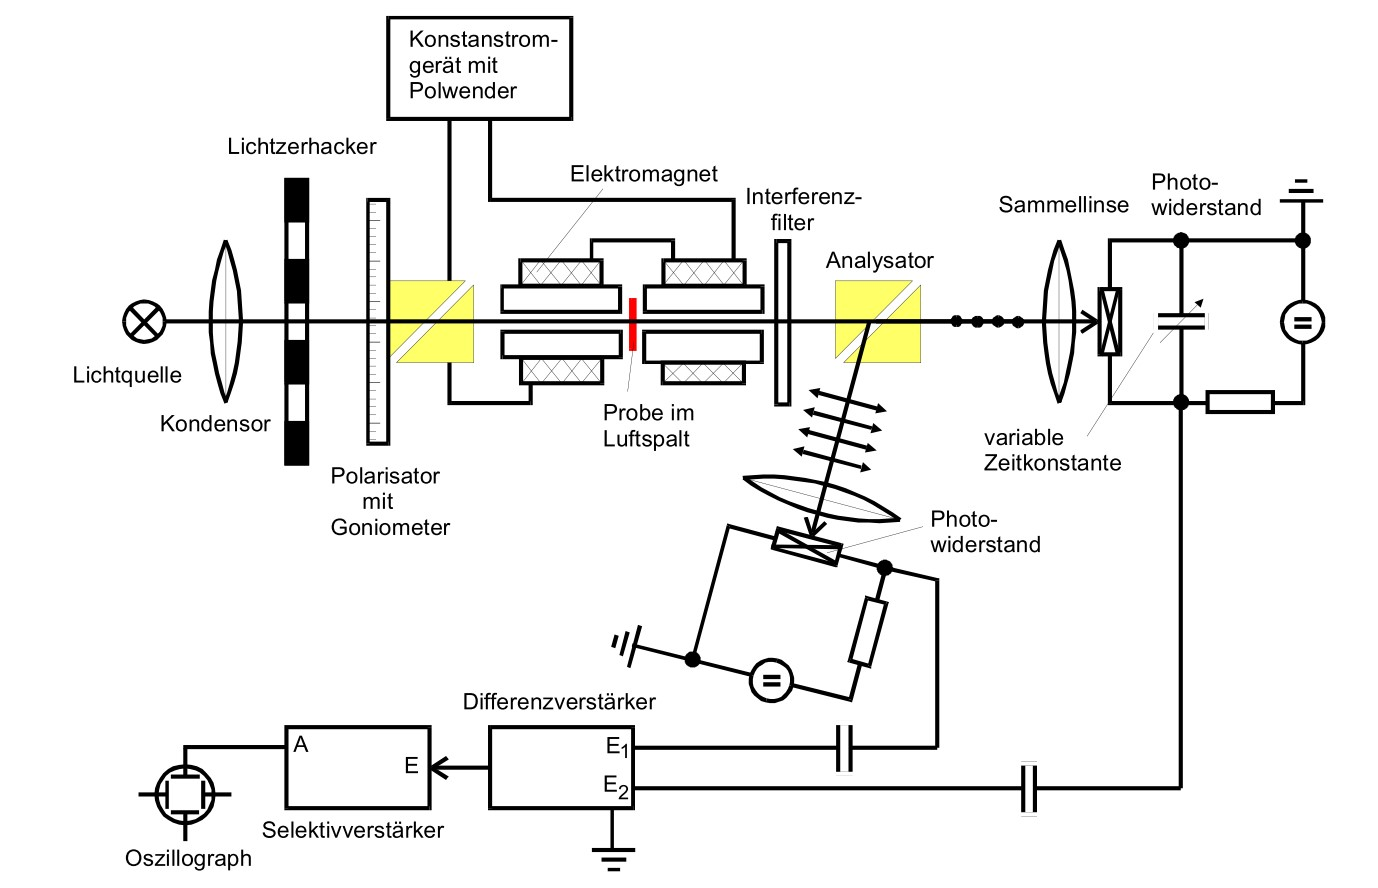
\includegraphics[width=0.8\textwidth]{figure/aufbau.jpg}
    \caption{Schematische Darstellung des Versuchaufbaus zur Bestimmung der effektiven Masse von Leitungselektronen mittel Faraday-Rotation. \cite{anleitung}}
    \label{fig:aufbau}
\end{figure}
Eine Halogen-Lampe emittiert Licht im sichtbaren bis Infrarot-Bereich.
Mithilfe einer Linse (Kondensor) wird der Lichtstrahl parallelisiert und auf den Lichtzerhacker abgebildet.
Als Lichtzerhacker wird eine rotierende Sektorscheibe bezeichnet.
Dieser \glqq zerstückelt\grqq den Lichtstrahl in Lichtimpulse, dabei kann die Frequenz eingestellt werden.
\\
Die Lichtimpulse treffen auf ein Glan-Thompson-Prisma, das hier die Funktion eines Polarisators hat.
Linear polarisiertes Licht (parallel zur optischen Achse des Prismas) tritt aus dem Polarisator aus und trifft auf die Probe.
Es existiert ein weiterer Lichtstrahl mit senkrecht zur optischen Achse linear polarisiertem Licht.
Dieser tritt aus dem Prisma aus und erfüllt keine weitere Funktion in diesem Aufbau.
Das Glan-Thompson-Prisma kann dabei um die optische Achse gedreht werden und der Rotationswinkel $\theta$ von einem Goniometer abgelesen werden.
\\
Die Probe befindet sich in einem Luftspalt zwischen zwei Magneten, die mit einem Konstantstromgerät gespeist werden.
Das Magnetfeld verläuft entlang der Flugrichtung der Photonen.
Als Probe liegt eine hochreine und zwei n-dotierte Galliumarsenid-Proben in Form einer Scheibe vor, die jederzeit ausgetauscht werden können.
\\
Der aus dem Medium austretende Lichtstrahl trifft auf einen Interferenzfilter.
Durch Verwendung verschiedener Interferenzfilter kann der Faraday-Effekt in Abhängigkeit der Wellenlänge untersucht werden.
\\
Ein weiteres Glan-Thompson-Prisma teilt den linear polarisierten Lichtstrahl in senkrecht und parallel polarisierte Anteile (im Bezug auf die optische Achse) auf.
Die Lichtstrahlen treffen jeweils auf eine Sammellinse, die das Bild scharf auf einen Photowiderstand aus dem Material PbS abbildet.
Der elektrische Widerstand ist dabei proportional zur Lichtintensität.
Eine Konstantspannungsquelle ist über einen Vorwiderstand an den Photowiderstand angeschlossen und es wird der Spannungsabfall gemessen.
Über einen Kondensator wird die Wechselspannung (verursacht durch den Lichtzerhacker) ausgekoppelt.
\\
Die Signalspannungen beider Photowiderstände werden auf die Eingänge eines Differenzverstärkers gegeben.
Dabei ist das Ausgangssignal proportional zu der Differenz der beiden gemessenen Spannung bzw. Lichtintensitäten.
Stimmt die Ausrichtung des ersten Glan-Thompson-Prisma (Rotationswinkel $\theta$) mit der Faraday-Rotation überein, so ist die Differenz minimal.
Es wird mit hoher Auflösung festgestellt ob die von den Photowiderständen gemessenen Intensitäten gleich sind.
\\
Die großen Widerstände in den Photodetektoren ($~\qty{1}{\mega\ohm}$) verursachen Rauschspannungen.
Um Untergrundsignale zu reduzieren wird die Wechsellichtmethode verwendet.
Das Ausgangssignal des Differenzverstärkers wird in ein Selektivverstärker gegeben.
Dieser verstärkt ein schmales Frequenzband, wobei die Frequenz an dem Verstärker eingestellt wird.
Sie sollte mit der Frequenz des Lichtzerhackers übereinstimmen.
\\
Das Ausgangssignal des Selektivverstärkers wird auf einem Oszilloskop visualisiert.
\\
\\
%Durchführung
Nach der Justierung des Strahlengangs, beginnt die Messung der Faraday-Rotation.
Bei maximal eingestelltem Magnetfeld wird der Winkel $\theta_1$ des ersten Glan-Thompson-Prismas so eingestellt, dass die Differenz der Signale beider Photowiderstände auf dem Oszilloskop minimal ist.
Anschließend wird das Magnetfeld umgepolt und erneut der Winkel $\theta_2$ variiert und gemessen.
\\
Für neun verschiedene Wellenlängen wird die Faraday-Rotation gemessen.
Dazu werden die gewünschten Interferenzfilter mit Wellenlängen im Bereich $\qty{1.07}{\micro\metre}$ bis $\qty{2.65}{\micro\metre}$ in die vorgesehene Stelle im Aufbau (siehe \autoref{fig:aufbau}) eingesetzt.
\\
Zum Schluss wird mit einer Hall-Sonde die Magnetfeldstärke im Bereich der Probe ermittelt.